

\documentclass{beamer}
\beamertemplatenavigationsymbolsempty

\usepackage[utf8]{inputenc}         % Input encoding (allow direct use of special characters like "ä")
%\usepackage[english]{babel}
\usepackage[ngerman]{babel}
\usepackage[T1]{fontenc}
\usepackage[automark]{scrpage2} 	 % Schickerer Satzspiegel mit KOMA-Script
\usepackage{setspace}           	 % Allow the modification of the space between lines

\usepackage{pdfpages}
% Um .eps Files einzubinden 
\usepackage{epstopdf} 

\AtBeginSubsection[]
{
  \begin{frame}
    \frametitle{Table of Contents}
    \tableofcontents[currentsection,currentsubsection]
  \end{frame}
}

\AtBeginSection[]
{
  \begin{frame}
    \frametitle{Table of Contents}
    \tableofcontents[currentsection]
  \end{frame}
}

\setbeamercovered{transparent}
\beamertemplatenavigationsymbolsempty
\setbeamertemplate{footline}[frame number]

\usetheme{Madrid}

\title[Seminar]{IT-Sicherheit Seminar}
\subtitle[Remailer]{Remailer: Typ-I bis Typ-III}
\author[M. McCreight]{Mervyn McCreight}
\institute[FH-Wedel]{FH-Wedel}

\subject{Remailer}
\keywords{Remailer, IT, Security, Anonymous, Pseudonymous}

\begin{document}

\frame{\titlepage}

\section{Cypherpunk-Remailer}
\begin{frame}
	\frametitle{Cypherpunk-Remailer}
	\begin{block}{Wesentliche Eigenschaften}
		\begin{itemize}
			\item Klassifizierung: Typ-I Remailer
			\pause
			\item "Cipher", "Cyber", "Punk"
			\pause
			\item Anonymisierend
			\pause
			\item Inspiration: Mix-Netzwerke \textit{(David Chaum)}
		\end{itemize}
	\end{block}
\end{frame}

\begin{frame}
	\begin{block}{Basis des Protokolls}
		Netzwerk von mehreren verschiedenen Cypherpunk-Remailern
	\end{block}
	\begin{columns}[T]
		\begin{column}[T]{5cm}
			\begin{center}
			Cypherpunk-Remailer \(C\) \\   

			\begin{figure}
			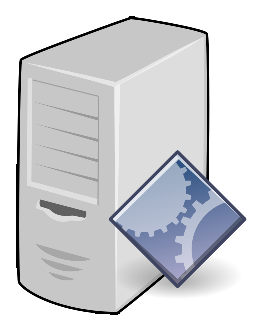
\includegraphics[height=3cm]{bilder/remailer.eps}
			\end{figure}
			\end{center}
		\end{column}
		\begin{column}[T]{5cm}
			\begin{center}	
			\begin{itemize}
				\item öffentlicher Schlüssel \(D_{C}\)
				\item privater Schlüssel \(E_{C}\)
				\item Nachricht entschlüsseln und weiterleiten
			\end{itemize}	
			\end{center}
		\end{column}
	\end{columns}
\end{frame}


\end{document}